%%
% BIThesis 研究生学位论文模板 The BIThesis Template for Graduate Thesis
% This file has no copyright assigned and is placed in the Public Domain.
%%

\chapter{相关理论与关键技术}
\label{chap:theory}

\section{知识图谱相关理论}

\subsection{知识图谱基本概念}

在众多可用于增强语义理解与知识组织的辅助信息中，知识图谱因其能够显式表示实体及其关系，逐步成为相关研究中的重要对象。该概念最早由 Google 公司提出，主要用于提升搜索引擎对语义化查询意图的理解和结果组织能力。从本质上看，知识图谱是一种结构化的语义网络，由节点和边组成\cite{Hogan2021KnowledgeGraphs}。在这一表示框架中，节点通常对应现实世界中的具体对象或抽象概念，边则用于刻画不同实体之间的语义联系。知识图谱中的事实知识一般可被表示为“实体—关系—实体”或“实体—边—实体”的三元组结构，从而使分散知识具备统一的结构化表达形式。通过这种方式，知识图谱能够有效地将用户和物品的属性信息、实体之间的关联信息以及用户与物品的行为信息组织起来，作为推荐系统的重要信息来源，从而提高推荐结果的准确性和多样性，并为推荐结果提供可解释路径。

以电影推荐场景为例，假设用户对影片“霸王别姬”表现出偏好，系统便可以沿着知识图谱中已有的实体关系进行关联扩展。例如，“阿飞正传”可通过主演关系与其建立联系，“末代皇帝”可通过题材关系与其关联，“搜索”则可通过导演关系与其相连。基于这些显式关系路径，推荐系统能够将与用户兴趣相关的候选影片组织起来，并据此生成更具解释性的推荐结果。如图~\ref{fig:kg-example}所示，图中的圆点代表实体，连线代表实体之间的关系，知识图谱正是通过这种显式关系组织方式，将原本分散的信息连接起来，形成可计算、可检索、可推理的知识网络。

\begin{figure}[htbp]
  \centering
  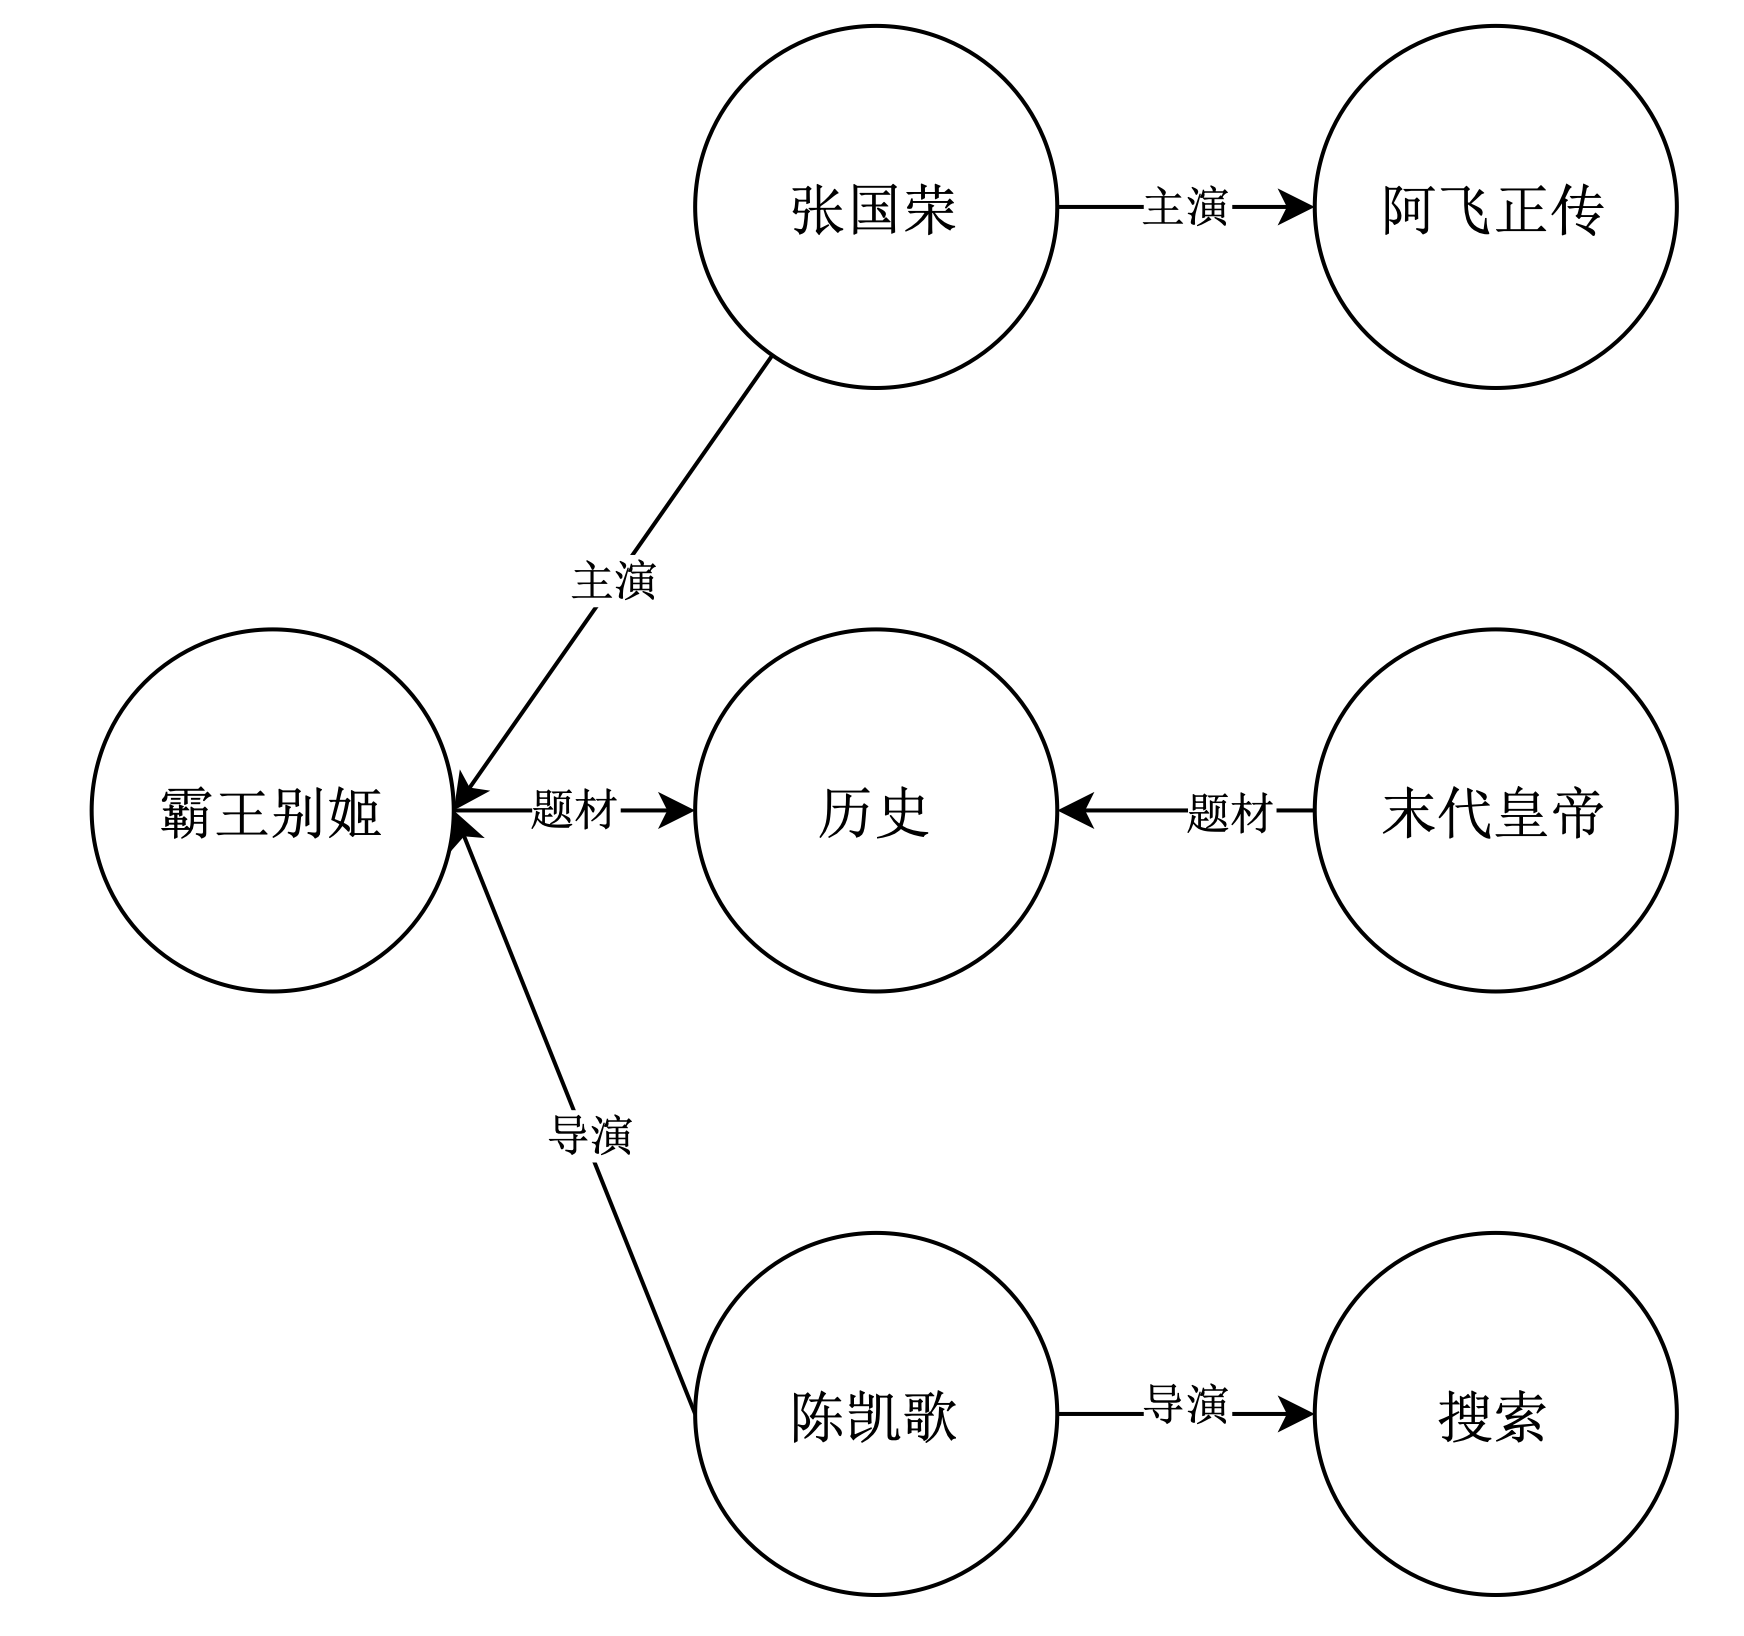
\includegraphics[width=0.7\textwidth]{figures/知识图谱示例.png}
  \caption{知识图谱示例}
  \label{fig:kg-example}
\end{figure}

知识图谱的形成通常依赖多个技术环节的协同作用。具体而言，知识抽取负责从开放数据或领域文本中识别实体、属性及实体间关系；知识融合用于处理不同来源知识在命名、指代或语义定义上的不一致；知识推理则能够在已有图谱基础上发现潜在关联或补充隐含知识，从而进一步扩展图谱内容\cite{Zhong2023AutomaticKGConstructionSurvey}。随着相关研究和工程实践的推进，知识图谱在语义表达、知识互联和关系组织方面的优势逐渐显现，并已被应用于个性化推荐、知识问答和智能检索等典型场景。就开放领域而言，Freebase、DBpedia 和 YAGO 等知识库是较具代表性的知识图谱资源\cite{Bollacker2007Freebase,Bizer2009DBpedia,Suchanek2008YAGO}。除开放领域知识库外，面向专业任务的领域知识图谱也逐渐形成了较多应用实践，如中药领域的 HerbNet、乳腺癌相关知识图谱以及数学知识库 WolframAlpha 等。由此可以看出，知识图谱的应用范围已不再局限于通用知识组织，而是逐步延伸至具有明确任务目标和专业语义约束的领域场景\cite{AbuSalih2021DomainSpecificKGSurvey}。

\subsection{知识图谱构建流程}

知识图谱的构建并不是简单地将若干实体和关系拼接在一起，而是一个从原始数据到结构化知识再到下游应用逐步演化的过程。从整体上看，知识图谱构建通常围绕知识获取、知识融合、知识存储和知识推理等环节展开；在具体实现中，又会进一步细化为数据获取、知识建模、知识抽取、融合管理和平台应用等多个阶段 \cite{Zhong2023AutomaticKGConstructionSurvey,Hogan2021KnowledgeGraphs}。这些环节相互衔接，共同决定了知识图谱的质量、可扩展性以及后续应用效果。

\begin{figure}[htbp]
  \centering
  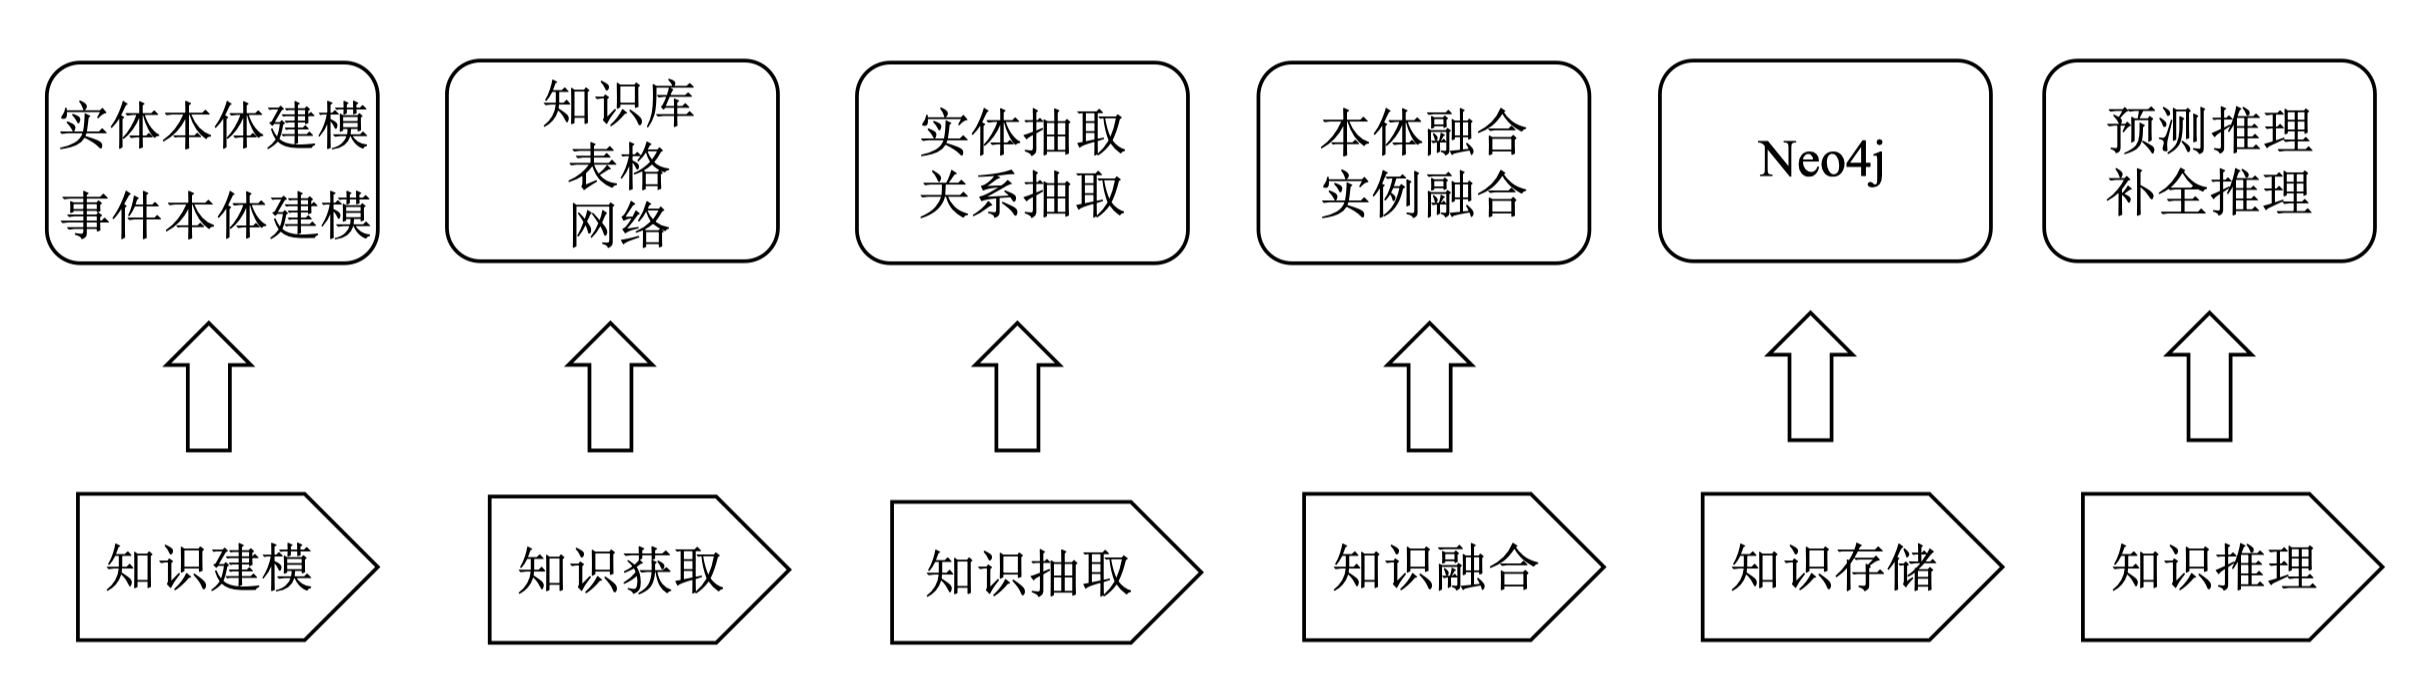
\includegraphics[width=0.9\textwidth]{figures/知识图谱构建流程.png}
  \caption{知识图谱构建流程}
  \label{fig:kg-construction-flow}
\end{figure}

图~\ref{fig:kg-construction-flow}展示了知识图谱构建的一般流程。该流程通常由知识获取、知识融合、知识存储和知识推理等环节构成。其中，知识获取位于流程前端，主要面向书籍、表格、文本语料等不同类型的数据源，通过知识抽取和知识建模等操作，将原始数据逐步转化为可用于图谱构建的结构化知识。知识抽取主要包括实体抽取和关系抽取等任务，用于从原始数据中识别关键对象及其联系；知识建模则进一步对实体、关系和属性进行抽象定义，在一些场景下还会涉及实体本体建模和事件本体建模，以保证后续图谱结构具有稳定的语义约束。

从任务定义角度看，领域知识图谱构建首先需要在给定文本中识别可构成关系的实体对象，并判断不同实体之间是否存在预设的语义联系，进而将抽取结果组织为图谱中的节点与边。该过程并不是简单地对文本中的关键词进行识别，而是要将非结构化文本中隐含的实体、关系及其语义联系转化为结构化三元组，从而为后续知识融合、图谱存储和下游应用提供基础。对于以军事新闻、医学文本、科学文档等为代表的垂直领域语料而言，这一过程尤其重要，因为这类文本通常具有较强的专业性、术语密集性和表达差异性，往往需要通过结构化处理才能被稳定组织和利用。

对于输入的长度为 $L$ 的领域文本序列
\begin{equation}
S=\{s_1,s_2,\ldots,s_L\},
\end{equation}
需要从中抽取若干个三元组，每个三元组包含两个实体和一个关系，即
\begin{equation}
\tau_i=(e_{i1},r_i,e_{i2}),
\end{equation}
其中，
\begin{equation}
e_{i1}=\{s_j,\ldots,s_k\}, \quad 0<j\leq k\leq L,
\end{equation}
\begin{equation}
e_{i2}=\{s_{j'},\ldots,s_{k'}\}, \quad 0<j'\leq k'\leq L,
\end{equation}
表示领域文本中蕴含的两个实体，而
\begin{equation}
r_i \in R
\end{equation}
表示预先定义的关系集合中的某一关系。换言之，知识图谱构建的核心任务，就是发现领域文本中包含的所有实体对，并确定它们之间的语义关系，再将其组织为后续可入库、可查询、可维护的结构化知识单元。

\begin{figure}[htbp]
  \centering
  % 请将下面的文件名替换为你保存的原图路径
  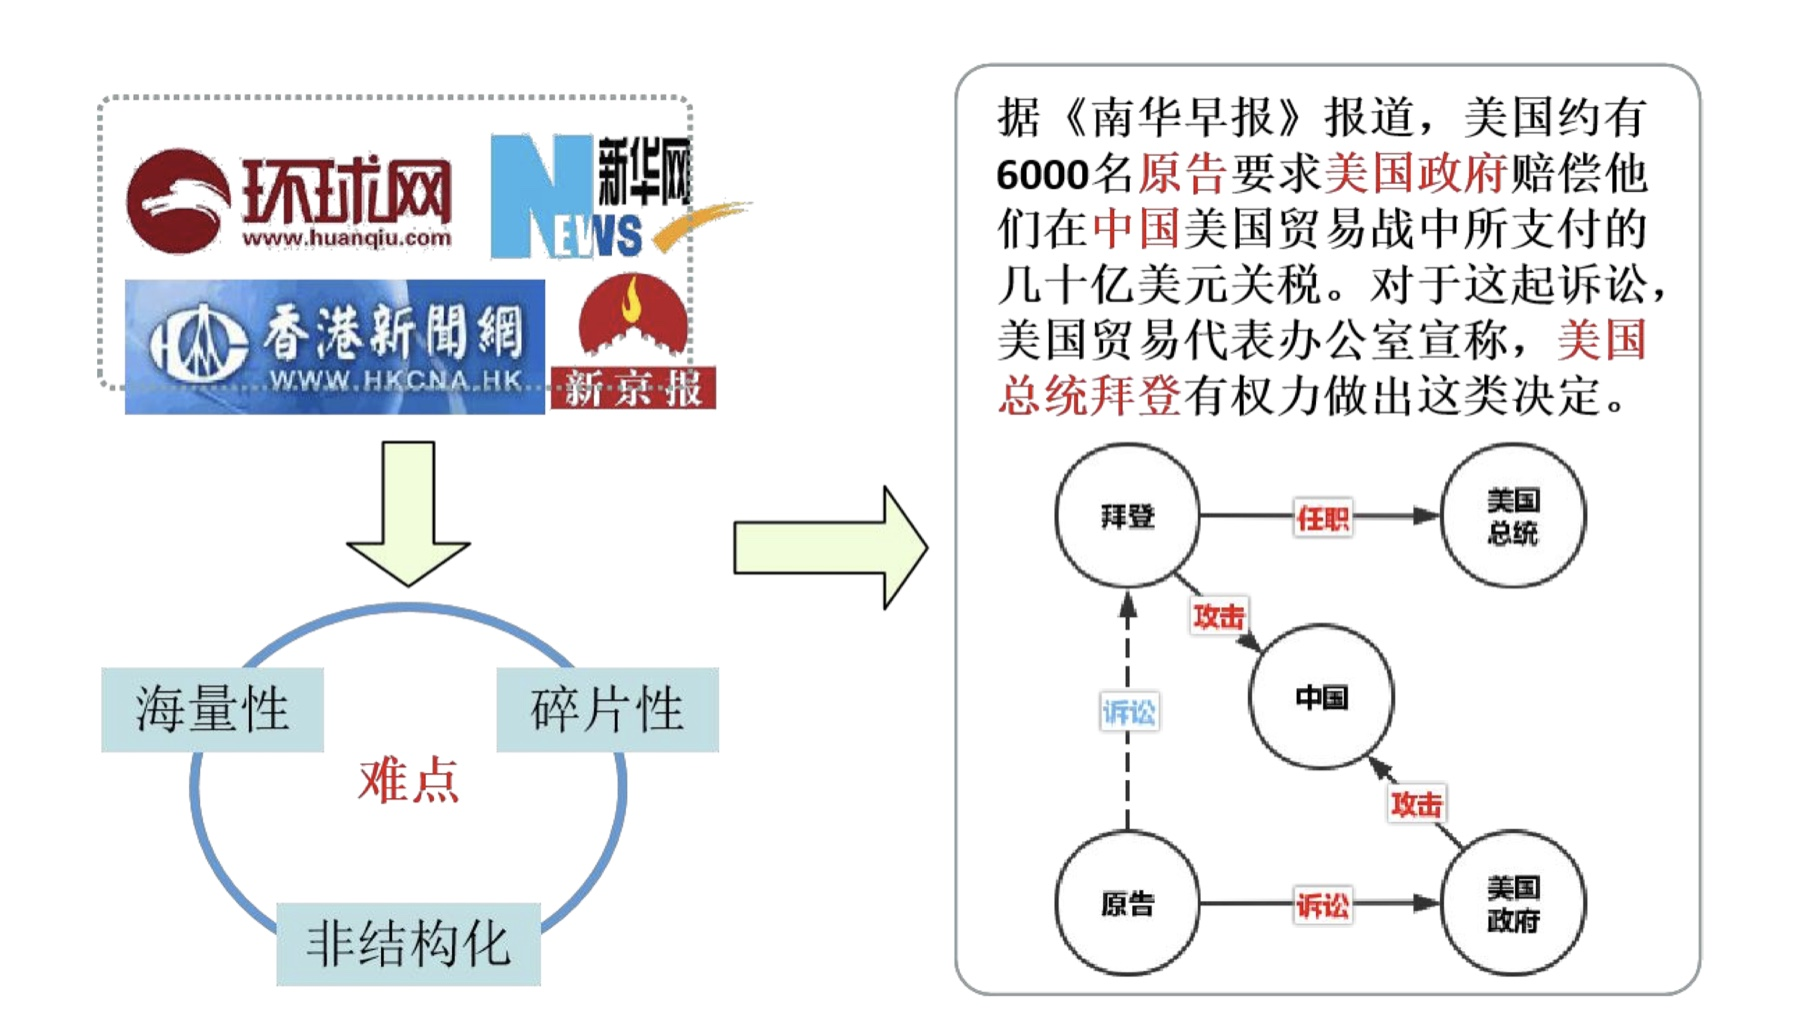
\includegraphics[width=0.9\textwidth]{figures/面向新闻领域的知识图谱构建示例已压缩.jpg}
  \caption{以新闻文本为例的垂直领域知识图谱构建示意}
  \label{fig:news-kg-construction-example}
\end{figure}

以新闻类领域语料为例，其知识图谱构建流程可参见图~\ref{fig:news-kg-construction-example}。该流程通常以相关文本采集为起点，即围绕目标主题从新闻网站等来源获取语料；随后通过分句、去重和人工审核等处理步骤完成初步清洗，并形成后续知识抽取与图谱构建所需的数据基础。进一步地，围绕新闻文本中出现的实体及其关系进行分析，将原本分散在自然语言中的知识转化为结构化表示。例如，对于新闻文本中的人物、机构、地点及其行为或属性关系，经过识别、建模与抽取后，可以形成若干“头实体—关系—尾实体”的三元组，并进一步写入知识图谱。通过这种方式，知识图谱构建流程就从“原始文本处理”推进到“结构化知识生成”，进而与后续的融合、存储和应用环节衔接起来。

在获得初步结构化知识后，还需要通过知识融合消除多源数据中的冗余和歧义。该过程通常包括本体融合和实例融合两个方面：前者侧重统一概念层面的模式定义，后者侧重对齐不同来源中的同名异义、异名同义和重复实体。完成冗余消解和实体对齐后，图谱知识可采用资源描述框架（Resource Description Framework，RDF）三元组等标准形式进行表示，并结合 Jena、Neo4j 等工具完成存储、可视化与管理，从而支撑知识库的查询、维护和后续应用。在此基础上，还可以通过预测推理、补全推理等方式进一步挖掘隐含知识，增强图谱的语义表达能力和应用价值。

首先是数据获取阶段。知识图谱构建的数据来源通常具有多源异构特征，既可以来自书籍、表格、数据库等结构化或半结构化数据，也可以来自网页文本、百科词条、领域文档等非结构化数据。在这一阶段，任务的关键是围绕目标领域筛选可用数据源，并完成数据收集、清洗和预处理，为后续建模和抽取提供输入。对于领域知识图谱而言，数据获取不仅要求覆盖领域核心实体和关系，还要求尽量保证数据的真实性、完整性和时效性，否则后续构建出的图谱容易出现知识缺失或语义偏差。

其次是知识建模与知识抽取阶段。知识建模的作用是从领域需求出发，对实体、关系和属性进行抽象定义，明确图谱中“有哪些对象”“对象之间存在哪些联系”以及“对象具备哪些属性”。在一些场景中，还需要进一步进行实体本体建模和事件本体建模，以形成更稳定的知识表示框架。在建模完成后，需要通过知识抽取将原始数据转化为结构化知识。对于文本数据而言，这一过程通常包括实体抽取和关系抽取两个核心步骤；对于表格、数据库等数据，则需要完成字段映射、语义对齐和结构转换。知识建模决定了知识图谱的结构边界，而知识抽取则决定了图谱中知识内容的具体来源和质量。

在抽取出初步知识之后，还需要进行知识融合。由于多源数据在命名方式、表达粒度和语义范围上往往存在差异，直接将其汇入同一图谱会产生大量重复实体、歧义关系和不一致描述。因此，知识融合通常需要在本体层和实例层两个层面展开：前者关注概念体系、关系模式和属性定义的一致性，后者关注实体对齐、名称归一化和重复实例合并。通过知识融合，可以提升图谱的统一性和可用性，使不同来源的知识能够在同一语义框架下被组织和管理。

完成融合之后，知识图谱需要进入知识存储与管理阶段。常见的表示方式是采用资源描述框架（Resource Description Framework，RDF）三元组对实体及其关系进行表达，并借助图数据库或语义存储工具实现管理和查询。在工程实现中，Jena 常用于 RDF 数据管理与语义处理，Neo4j 则常用于图结构数据的存储、可视化和关系查询。通过这一阶段，原本分散的数据与抽取结果被组织为可维护的知识图谱，为后续检索、分析与服务平台接入提供基础。

最后是知识推理与平台应用阶段。知识推理的目标是在已有知识图谱的基础上发现潜在关联，补全隐含知识，并支持更高层次的语义计算。常见形式包括预测推理和补全推理等。经过推理增强后的知识图谱可以进一步支撑推荐系统、智能问答、知识检索、辅助决策等应用场景。换言之，知识图谱构建流程并不是在图谱生成后结束，而是要通过管理、推理和应用形成闭环，使图谱从“可存储的结构化知识”进一步转化为“可服务的智能基础设施”。这一路径也为本文后续讨论面向领域知识图谱构建的知识抽取与应用实现提供了流程层面的理论基础。
\section{知识抽取相关技术}

\subsection{命名实体识别}

命名实体识别（Named Entity Recognition，NER）是实体抽取任务中的基础环节，主要用于从自然语言文本中定位并识别具有特定语义类别的实体对象，如人名、专业名称、职业名称等。在知识图谱构建流程中，命名实体识别承担着确定图谱节点候选对象的作用，其结果会进一步影响关系抽取、实体对齐以及知识入库等后续环节。因此，NER 的识别准确性与边界判定质量，在很大程度上决定了图谱构建结果的可靠性。根据技术路线和方法演进过程，现有命名实体识别方法大致可归纳为以下四类。

第一类为基于规则和词典的命名实体识别方法。这类方法多见于早期研究，其基本流程是由领域专家预先构建实体词典、类别定义和匹配规则，再利用这些规则对文本进行扫描与匹配，并将命中的实体划分到相应类别中。在语料规模较小、实体类型相对固定的场景下，该方法通常能够取得较稳定的识别效果；但由于规则设计、词典维护和类别扩展高度依赖人工经验，当数据规模扩大或文本表达更加多样时，其维护成本会显著上升，适用范围也随之受限。

第二类为基于传统机器学习的命名实体识别方法。与规则词典方法相比，这类方法通常将 NER 建模为监督学习或序列标注问题：首先在训练语料中人工标注实体边界和类别，例如采用 BIO 标注体系表示实体的起始、内部和非实体位置；随后围绕词语、上下文及句法等信息构造特征，并在此基础上训练分类模型或序列标注模型。训练完成后，模型即可将学习到的标注模式迁移到未标注文本中，用于识别新的命名实体。在传统机器学习框架下，命名实体识别常采用隐马尔可夫模型（Hidden Markov Models，HMM）、决策树（Decision Trees，DT）、支持向量机（Support Vector Machines，SVM）以及条件随机场（Conditional Random Fields，CRF）等模型实现\cite{Rabiner1989HMMTutorial,Quinlan1986DecisionTrees,Chen2005NuSVM,Sutton2012CRFTutorial}。其中，CRF 能够对序列标签之间的转移关系进行建模，因此在早期 NER 任务中应用较为广泛。在深度学习方法逐渐应用于自然语言处理任务后，CRF 往往不再单独使用，而是作为序列标签约束层与神经网络模型结合，服务于分词、命名实体识别等需要连续标签预测的任务。

第三类为基于传统深度学习的命名实体识别方法。相较于依赖人工特征设计和外部词典的传统机器学习方法，深度神经网络能够通过表示学习自动捕捉词语及上下文信息，因此逐渐被引入 NER 任务中，用于降低人工特征工程在模型构建中的比重。在深度学习用于命名实体识别的早期研究中，SENNA 是较具代表性的序列标注模型之一。该模型弱化了对人工特征工程的依赖，主要通过大规模未标注语料学习词语表示，并在此基础上训练深度前馈神经网络完成序列标注任务\cite{Collobert2011NLPFromScratch}。在 SENNA 等早期神经网络序列标注方法之后，研究者进一步将双向长短期记忆网络（Bidirectional Long Short-Term Memory，BiLSTM）引入命名实体识别任务，用于同时建模词语前后两个方向的上下文信息。为增强标签序列的整体一致性，模型通常在 BiLSTM 输出层之后接入条件随机场（Conditional Random Fields，CRF），由此形成双向长短期记忆网络-条件随机场模型（Bidirectional Long Short-Term Memory-Conditional Random Fields，BiLSTM-CRF）\cite{Lample2016NeuralArchitecturesNER}，其结构如图~\ref{fig:bilstm-crf}所示。

\begin{figure}[htbp]
  \centering
  % 后续可将下方占位框替换为你自己的图，例如：
  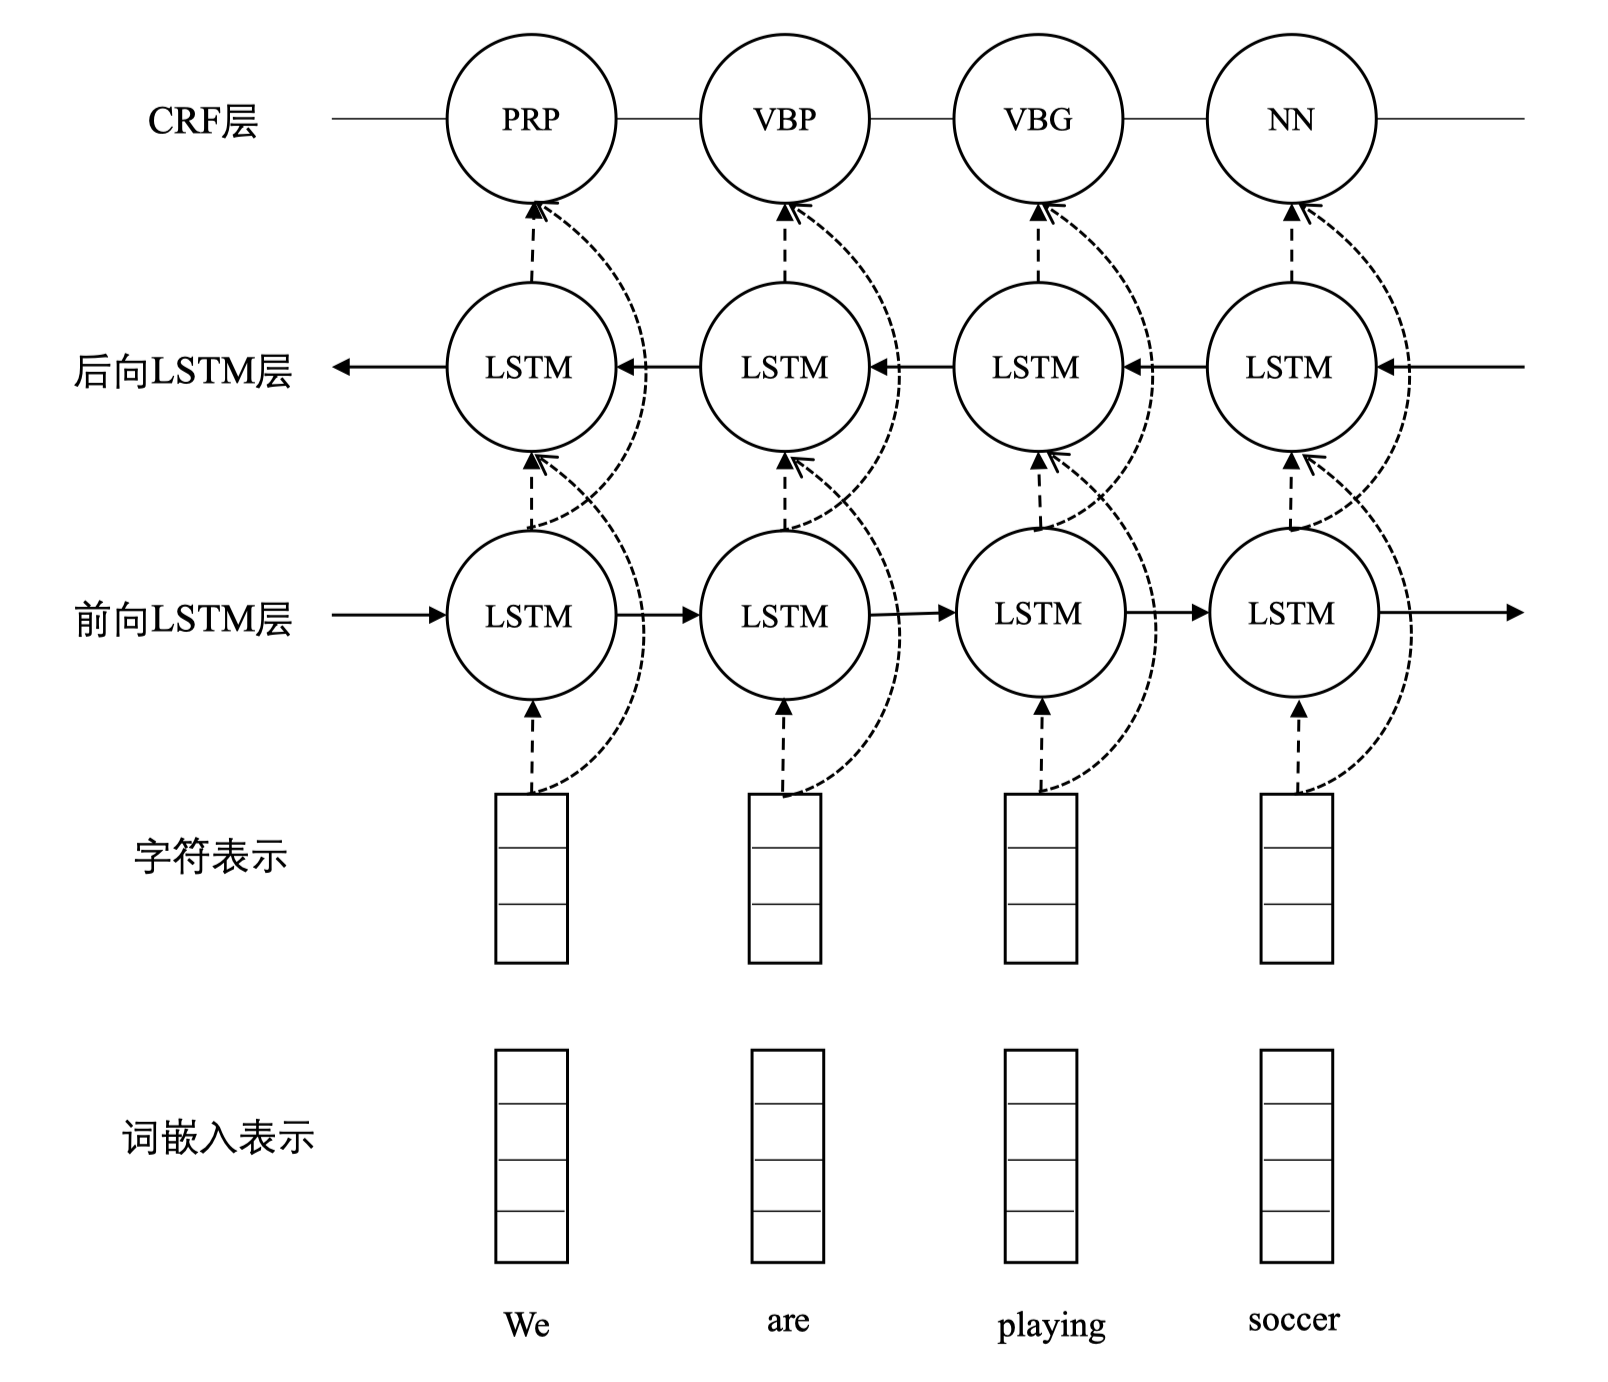
\includegraphics[width=0.8\textwidth]{figures/bilstm-crf.png}
  % \fbox{\parbox[c][5cm][c]{0.78\textwidth}{\centering 此处预留原文“图2.3”位置\\BiLSTM-CRF 模型示意图}}
  \caption{BiLSTM-CRF 模型示意图}
  \label{fig:bilstm-crf}
\end{figure}

由于能够同时利用上下文表示学习能力和标签转移约束，BiLSTM-CRF 已成为命名实体识别研究中的代表性神经网络模型，并在许多序列标注任务中表现出优于传统机器学习方法的效果。

第四类方法以 Transformer 架构为基础，代表模型包括双向编码器表示模型（Bidirectional Encoder Representations from Transformers，BERT）和生成式预训练变换器（Generative Pre-trained Transformer，GPT）。在当前命名实体识别研究中，BERT 及其变体仍是较常用的预训练语言模型框架。与早期面向单一任务训练的监督学习模型相比，BERT 和 GPT 系列模型首先通过大规模语料预训练获得通用语言表示，再根据情感分类、命名实体识别等具体任务进行适配。传统监督学习模型通常需要大量高质量标注数据，并且在不同任务和场景之间的迁移能力较弱，因此往往会带来较高的数据标注成本；而 BERT 和 GPT 系列模型在一定程度上缓解了这一问题。

BERT 的预训练过程主要依托大规模文本语料进行语言表示学习，其核心任务包括掩码语言模型（Masked Language Model，MLM）和下一句预测（Next Sentence Prediction，NSP）。其中，MLM 通过随机遮蔽输入序列中的部分词语，并要求模型根据上下文恢复被遮蔽内容，以学习双向语义表示；NSP 则通过判断两个给定句子之间是否具有连续关系，使模型获得一定的句间关系建模能力。由于这两个预训练任务可直接从原始文本中构造训练信号，因此不需要额外人工标注数据\cite{Devlin2019BERT}。在实际应用中，BERT 通常作为文本表示模型嵌入到不同下游任务框架中，例如情感分类、问答系统和命名实体识别等任务；在具体任务适配阶段，仍需要结合相应的标注数据进行监督训练。与之相比，GPT 系列模型更强调基于大规模混合语料的生成式预训练，通过学习通用语言模式提升模型在不同任务间的迁移能力，并在一定程度上降低对大规模人工标注数据的依赖。

从模型结构看，BERT 与 GPT 系列模型虽然在建模目标和使用方式上存在差异，但二者均建立在变换器（Transformer）架构之上\cite{Vaswani2017AttentionIsAllYouNeed}，其基本结构如图~\ref{fig:transformer-architecture}所示。Transformer 由编码器和解码器两部分构成，并以多头注意力机制（Multi-Head Attention）为关键计算模块；该机制结合自注意力机制（Self-Attention Mechanism，SAM）与位置编码（Positional Encoding），使模型能够在并行计算的同时建模序列中不同位置之间的依赖关系。

\begin{figure}[htbp]
  \centering
  % 后续可将下方占位框替换为你自己的图，例如：
  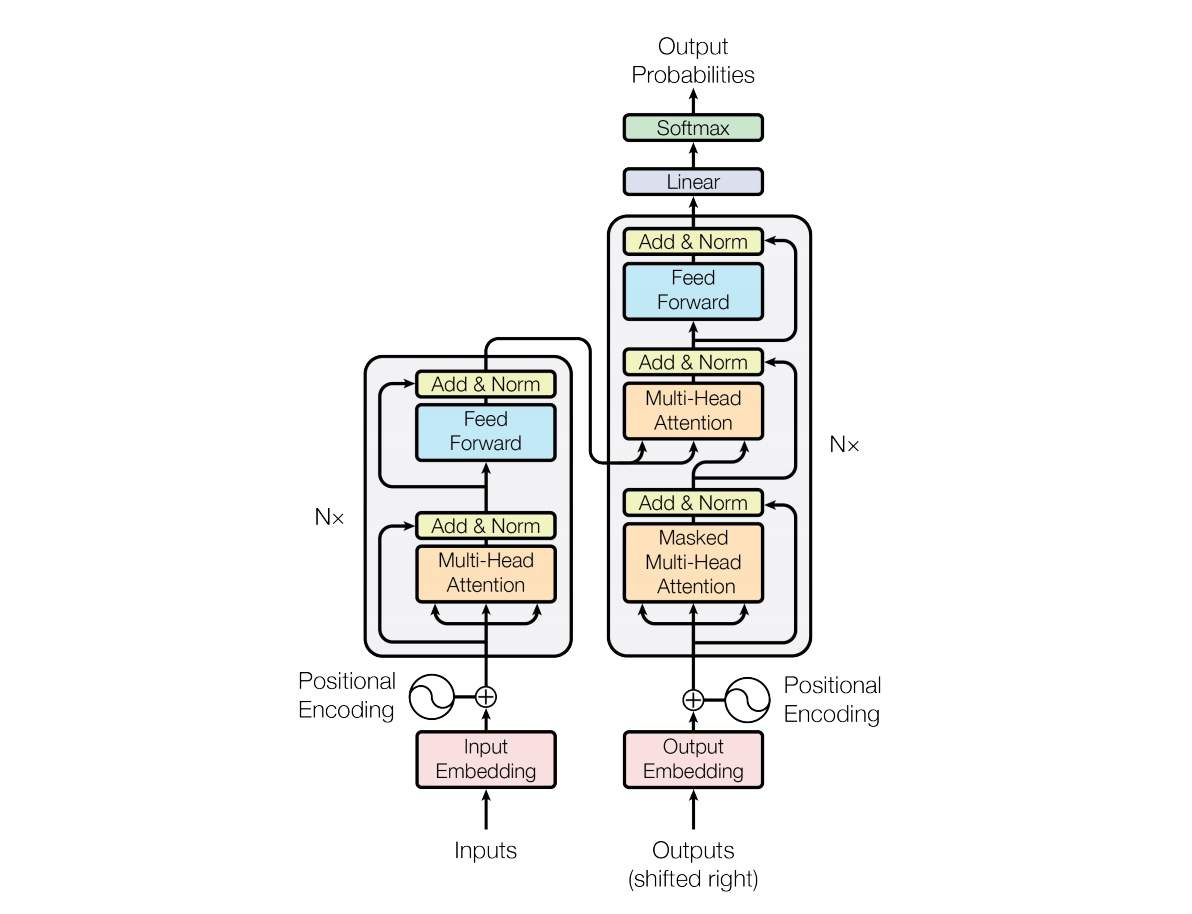
\includegraphics[width=0.9\textwidth]{figures/transformer-architecture.png}
  % \fbox{\parbox[c][5.2cm][c]{0.82\textwidth}{\centering 此处预留原文“图2.4”位置\\Transformer 模型结构图}}
  \caption{Transformer 模型结构图}
  \label{fig:transformer-architecture}
\end{figure}

在 Transformer 的计算流程中，输入序列通常先被映射为向量表示，并叠加位置编码，以弥补模型本身缺少顺序结构建模的不足。随后，多头注意力机制从不同表示子空间对序列信息进行交互建模，得到包含上下文关联的特征表示。前馈神经网络（Feed Forward Network）则进一步对这些特征进行非线性变换，形成更高层次的语义表示。在上述计算过程中，残差连接（Add）和层归一化（Layer Normalization）用于增强深层网络训练的稳定性。残差连接通过将前一层的输出与当前层的输出相加，有助于缓解深度神经网络训练过程中的梯度消失问题；而层归一化则通过对每一层的输出进行规范化，使模型在训练过程中保持较为稳定的性能。编码器和解码器都是由 $N$ 个相同层堆叠而成，源序列和目标序列数据经过嵌入层后会产生相同维度的表示。

BERT 采用 Transformer 的编码器部分作为主体结构。每个编码器层通常由多头注意力机制（Multi-Head Attention）和前馈神经网络（Feed Forward Network）组成，其中自注意力机制负责计算序列内部不同位置之间的关联，使模型在表示某一词语时能够同时利用其他位置的上下文信息；多头机制则通过设置多个注意力头，使模型从不同表示角度学习词语间的语义联系，并在合并各头结果后形成更完整的上下文表示。BERT 依托掩码语言模型（Masked Language Model，MLM）学习双向上下文语义，即在同时利用左右两侧语境的基础上恢复被遮蔽词语；同时，其通过下一句预测（Next Sentence Prediction，NSP）任务建模句子之间的连续关系，从而增强对篇章级语义关联的表示能力。由于 BERT 采用双向编码方式，如图~\ref{fig:bert-architecture}所示，其能够在生成词语表示时综合利用前后文信息，因此更适合文本分类、语义匹配和命名实体识别等理解类任务。在知识图谱构建场景中，NER 需要准确判定实体边界及其类别，因而 BERT 常被用作该类任务的语义表示基础。

\begin{figure}[htbp]
  \centering
  % 后续可将下方占位框替换为你自己的图，例如：
  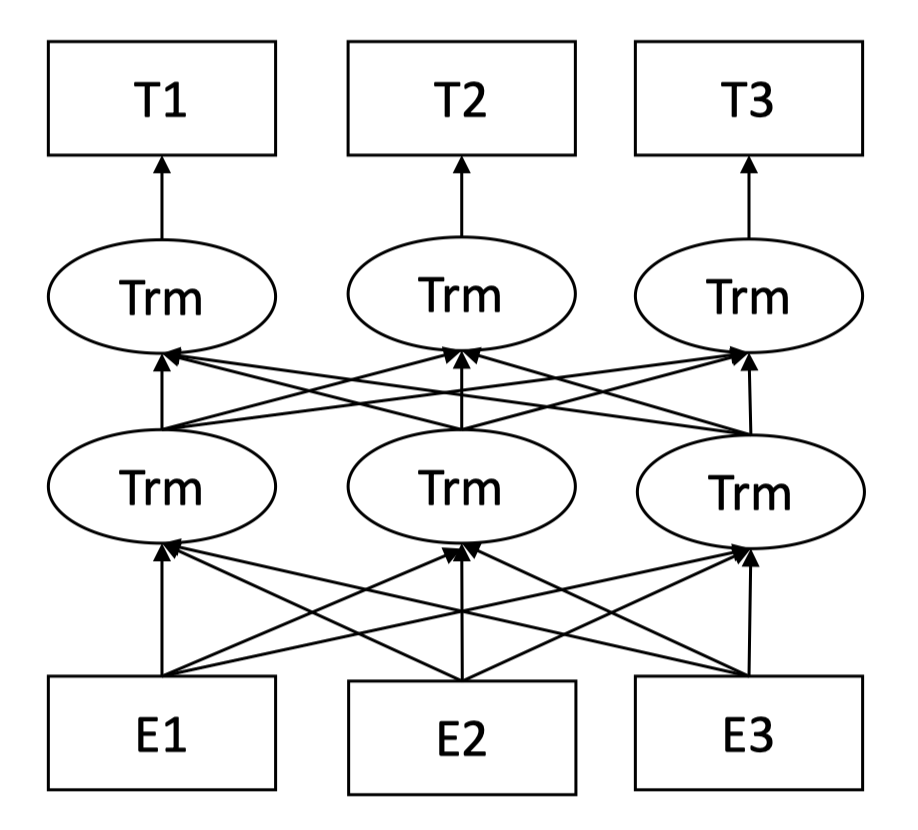
\includegraphics[width=0.55\textwidth]{figures/bert-architecture.png}
  % \fbox{\parbox[c][4.8cm][c]{0.56\textwidth}{\centering 此处预留原文“图2.5”位置\\BERT 模型架构}}
  \caption{BERT 模型架构}
  \label{fig:bert-architecture}
\end{figure}

与 BERT 主要采用编码器结构不同，GPT 系列模型以 Transformer 的解码器为核心。编码器在计算某一位置的表示时，通常可以同时利用输入序列中各位置的信息；而解码器引入了掩码机制，使模型在处理第 $i$ 个位置时只能访问当前位置及其之前的上下文，后续位置的信息会在注意力计算中被屏蔽。由此，GPT 的表示学习过程呈现出从左到右的自回归特征。如图~\ref{fig:gpt-architecture}所示，GPT 的单向建模机制使其能够按照自回归方式逐步生成文本，即根据已有上下文预测后续内容。因此，GPT 系列模型在摘要生成、机器翻译等生成式自然语言处理任务中具有较强适用性，并逐渐成为大语言模型发展的重要代表。在知识抽取任务中，大语言模型不仅能够承担文本理解与语义表示功能，也可以通过指令式生成方式参与结构化知识获取，包括命名实体识别、实体属性识别及相关抽取任务。随着生成式模型能力的提升，NER 的实现路径也不再局限于传统序列标注框架，而是逐步扩展到面向自然语言指令的生成式抽取范式\cite{Xu2024LLMGenerativeIESurvey}。

\begin{figure}[htbp]
  \centering
  % 后续可将下方占位框替换为你自己的图，例如：
  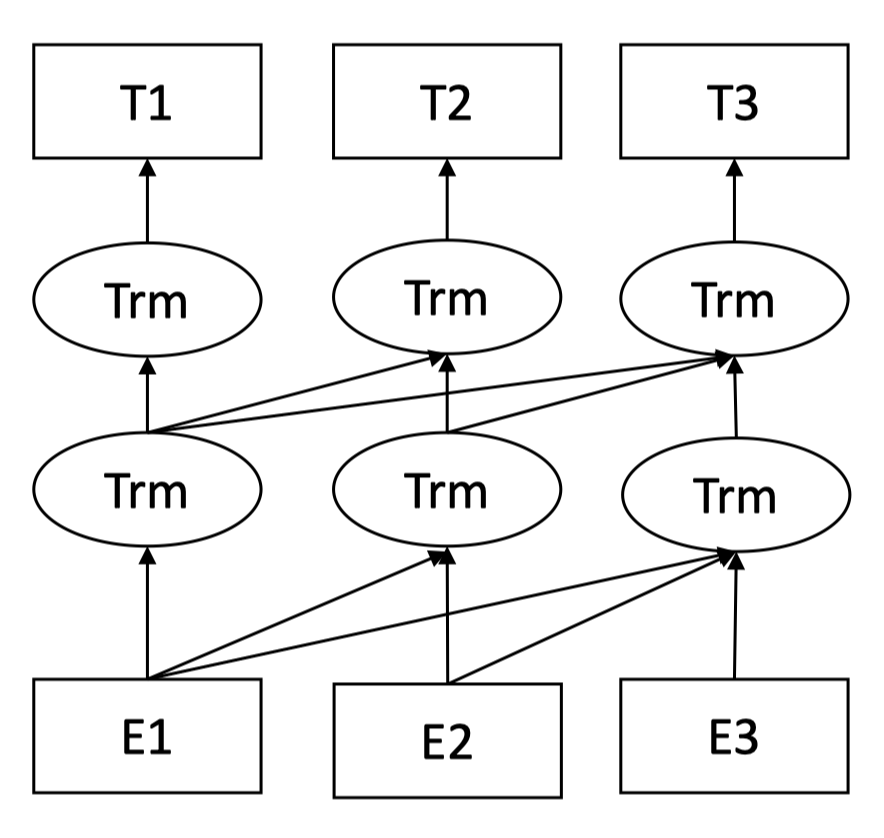
\includegraphics[width=0.55\textwidth]{figures/gpt-architecture.png}
  % \fbox{\parbox[c][4.8cm][c]{0.56\textwidth}{\centering 此处预留原文“图2.6”位置\\GPT 模型架构}}
  \caption{GPT 模型架构}
  \label{fig:gpt-architecture}
\end{figure}

综上，命名实体识别技术的发展大体呈现出由人工规则驱动向数据驱动、再向预训练语言模型驱动演进的趋势。规则词典方法强调人工知识约束，传统机器学习方法依赖特征设计与监督标注，深度学习方法进一步提升了上下文表示能力，而预训练语言模型则增强了模型在不同任务和领域中的迁移潜力。上述技术演进为后文研究面向领域知识图谱构建的可控知识抽取方法奠定了基础。

\subsection{关系抽取}

关系抽取是知识抽取中的重要任务，主要用于判断文本中已识别实体之间是否存在特定语义关联，并将这种关联转换为可被计算和存储的结构化关系表示。在知识图谱构建场景下，实体能否形成有意义的边，取决于关系抽取能否准确识别实体间的语义连接。因此，关系抽取不仅影响图谱中关系边的生成，也会进一步影响图谱结构的完整性和可用性。根据技术路线的演进，现有关系抽取方法大体可归纳为三种类型。

第一类为基于模板的关系抽取方法。这类方法多用于早期关系抽取研究，通常依赖人工或半自动构建的关系模式来匹配文本表达，具体可进一步划分为触发词匹配和依存分析匹配两种形式。在基于触发词的关系抽取方法中，通常需要先构造若干能够表达特定关系的种子模板，再利用这些模板与待处理文本进行匹配。以句子“[姚明]的妻子[叶莉]与他一起出席了活动”为例，可先将其中的人名统一替换为实体占位符，得到“[E1]的妻子[E2]”这一关系模式。随后，系统即可将“的妻子”识别为关系触发线索，并据此判断实体 [E1] 与实体 [E2] 之间存在“妻子”关系。除触发词匹配外，依存分析方法还可以借助句法结构识别实体之间的潜在关系，其一般处理流程见图~\ref{fig:dependency-pattern-workflow}。该方法通常先对输入句子进行分词、词性标注和命名实体识别等处理，再根据依存树上的匹配规则抽取子树结构；每匹配一条规则便生成一个候选三元组，之后结合扩展规则和评价机制形成关系抽取结果。基于模板的方法在较小数据集上的准确率较高，但随着数据集规模增大，人工编写模板的成本迅速上升，且对关系的覆盖不够全面，因此并不适用于大规模数据集的关系抽取。

\begin{figure}[htbp]
  \centering
  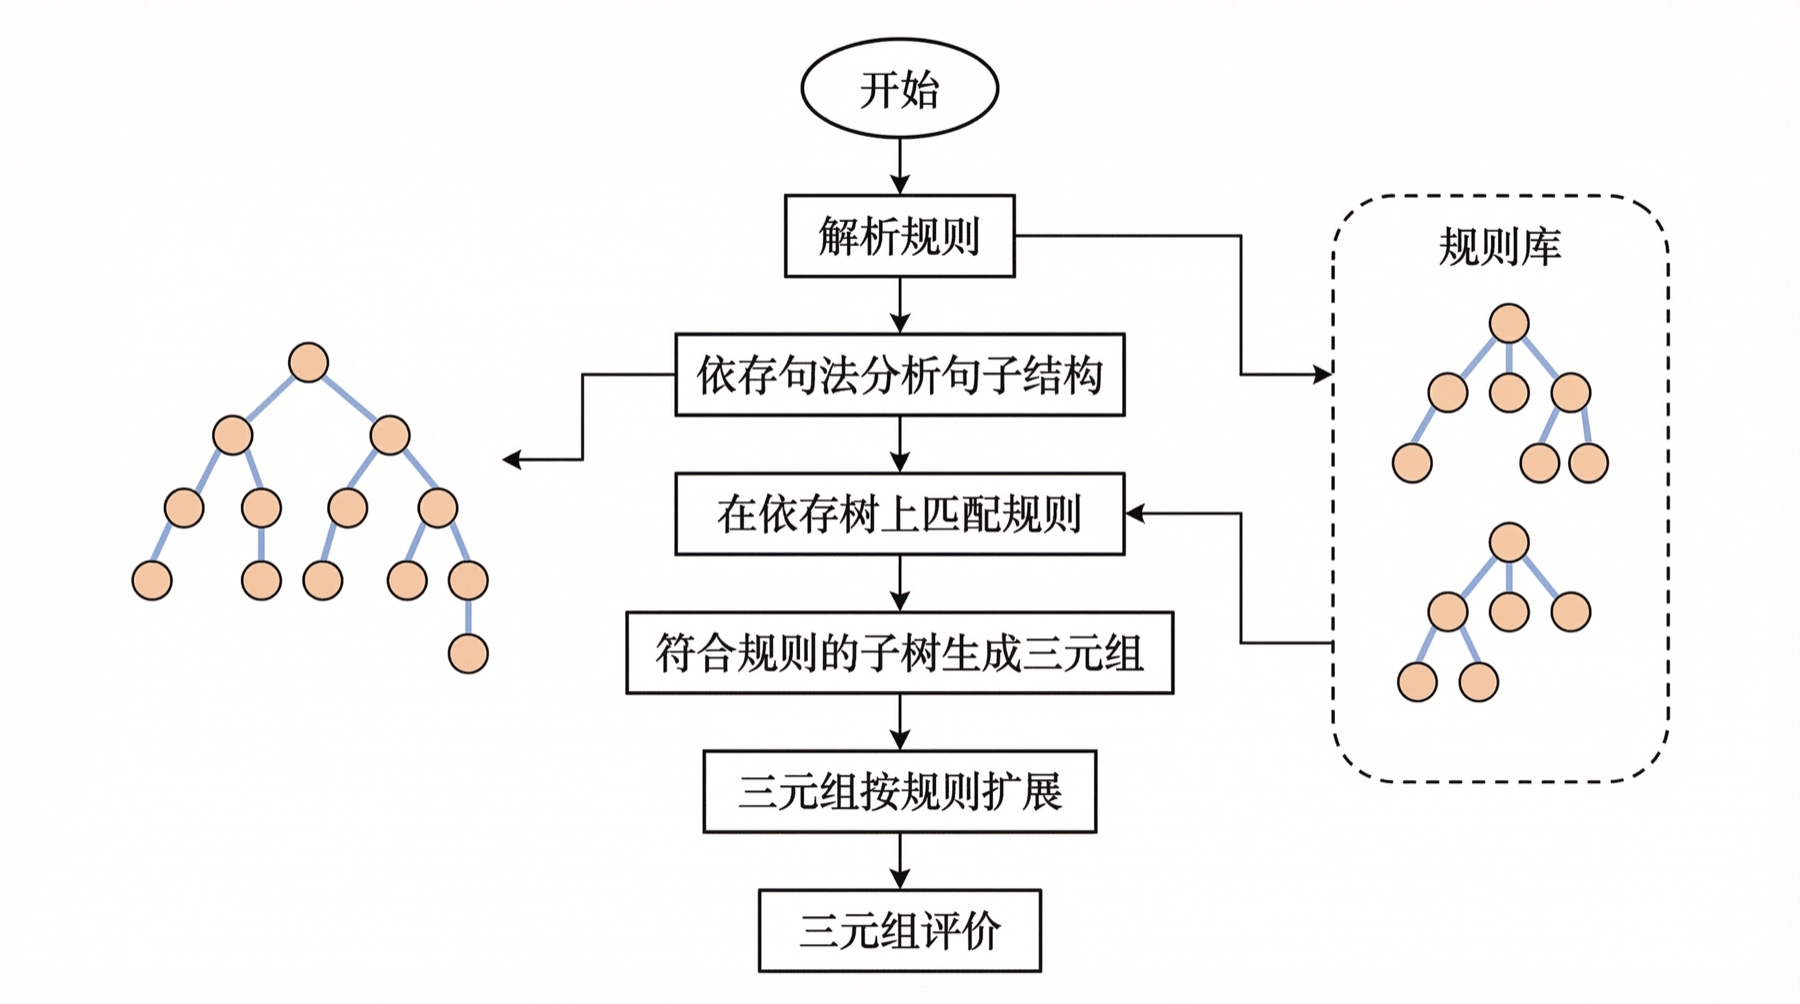
\includegraphics[width=0.9\textwidth]{figures/基于依存分析的模式流程已压缩.jpg}
  \caption{基于依存分析的模式流程}
  \label{fig:dependency-pattern-workflow}
\end{figure}

第二类为基于监督学习的关系抽取方法。这类方法通常把关系抽取建模为实体对层面的分类任务，即在已标注训练语料中给定实体对及其关系类别，再围绕上下文词汇、句法结构和语义信息构造特征表示，并通过分类模型学习不同实体对与关系类型之间的映射关系。常见的分类模型包括支持向量机（Support Vector Machines，SVM）和朴素贝叶斯（Naive Bayes）等\cite{Chen2005NuSVM,Zhang2004OptimalityNaiveBayes}。当训练样本规模较大且标注质量较高时，监督学习方法通常能够获得较稳定的关系识别效果。然而，该方法对人工标注语料的依赖较强，数据准备成本较高；同时，特征构造往往需要结合具体语料和领域经验进行设计，因此在跨领域应用时容易受到文本风格、关系类型和语义表达差异的影响。

第三类为基于弱监督学习的关系抽取方法，其中远监督是较具代表性的实现方式。远监督的基本假设是：若知识库中已经记录某一实体对之间存在特定关系，则包含该实体对的文本句子有可能表达相同关系。以“省会（杭州，浙江）”为例，当句子中同时出现“杭州”和“浙江”时，系统可依据知识库中的既有关系自动构造候选训练样例，用于学习“省会”关系的表达模式\cite{Mintz2009DistantSupervision}。远监督方法的优势在于能够借助知识库中的既有关联自动生成训练样本，从而降低人工逐条标注的成本。但由于“实体共现”并不必然意味着句子真实表达了知识库中的关系，该方法也容易产生噪声样本。例如，“杭州位于浙江东部”虽然同时包含“杭州”和“浙江”，但句子语义并未表达“省会”关系。此外，远监督方法的覆盖范围通常受已有知识库限制，对于知识库中尚未记录的新关系识别能力相对不足。

Bootstrapping 方法通常从少量种子实例出发，先构建初始关系实例集合，再依据这些种子实例归纳或匹配关系模板，并在文档中发现新的候选实例。新抽取出的实例会被继续加入集合中，参与后续轮次的模板扩展与实例匹配，直至迭代过程收敛或不再产生有效增量。该方法能够在较低标注成本下扩展关系实例规模，因而适用于较大规模文本集合中的关系抽取，并具备一定的新关系发现能力；但其效果容易受到初始种子质量影响，若早期样本存在偏差，后续迭代可能进一步放大错误，导致部分场景下准确率下降。总体来看，关系抽取方法经历了从基于模板的方法、基于监督学习的方法，到基于弱监督学习的方法的发展过程。不同方法在准确率、人工成本和可扩展性方面各有特点，也为后续基于深度学习和大语言模型的关系抽取研究奠定了基础。

\subsection{实体关系联合抽取}

实体关系联合抽取是知识图谱构建中的重要基础环节，其核心任务是在同一处理框架下识别领域文本中的实体对象，并判断实体之间是否存在预定义关系。通过这一过程，原本以自然语言形式存在的非结构化文本可以被转换为“头实体—关系—尾实体”的三元组知识单元，进而为图谱存储、查询以及下游知识服务提供结构化数据支撑。从任务组成来看，实体关系联合抽取通常同时包含实体抽取和关系抽取两个部分。实体抽取侧重于确定文本中的实体边界及其类别，关系抽取则进一步分析候选实体之间的语义联系，并判断其是否属于既定关系集合中的某一类型。

\begin{table}[htbp]
  \centering
  \caption{知识图谱构建示例，将非结构化文本转化为结构化三元组}
  \label{tab:joint_extraction_example}
  {\renewcommand{\arraystretch}{1.2}
  \begin{tabular*}{0.92\textwidth}{@{\extracolsep{\fill}}p{0.42\textwidth}p{0.46\textwidth}}
    \toprule
    输入文本 & 三元组 \\
    \midrule
    德国经济部长彼得$\cdot$阿尔特迈尔希望美国总统拜登上任后能够消除美欧间的贸易壁垒。
    &
    \begin{tabular}[t]{@{}l@{}}
    （彼得$\cdot$阿尔特迈尔，任职，德国经济部长） \\
    （拜登，任职，美国总统）
    \end{tabular}
    \\
    《我和我的祖国》是由陈凯歌担任总导演，张一白、薛晓路、徐峥、宁浩等人联合执导的剧情片，于 2019 年 9 月 30 日在中国大陆上映。
    &
    \begin{tabular}[t]{@{}l@{}}
    （陈凯歌，总导演，《我和我的祖国》） \\
    （张一白，导演，《我和我的祖国》） \\
    （薛晓路，导演，《我和我的祖国》） \\
    （徐峥，导演，《我和我的祖国》） \\
    （宁浩，导演，《我和我的祖国》）
    \end{tabular}
    \\
    \bottomrule
  \end{tabular*}}
\end{table}

表~\ref{tab:joint_extraction_example}给出了非结构化文本向结构化三元组转换的示例。以新闻文本“德国经济部长彼得$\cdot$阿尔特迈尔希望美国总统拜登上任后能够消除美欧间的贸易壁垒。”为例，模型需要先识别出“彼得$\cdot$阿尔特迈尔”“德国经济部长”“拜登”“美国总统”等实体或角色表达，再判断其间是否存在“任职”关系。经过实体识别与关系判定后，该句可被组织为“（彼得$\cdot$阿尔特迈尔，任职，德国经济部长）”和“（拜登，任职，美国总统）”等结构化三元组。通过上述方式，能够从海量领域文本中构建知识图谱，为有效利用文本中蕴含的丰富知识奠定基础。

现有实体关系联合抽取方法大体可以从建模方式上划分为两类：一类依赖人工设计特征和规则约束，通常被归入基于特征工程的方法；另一类则利用神经网络自动学习文本表示，属于基于神经网络的方法。进一步看，神经网络方法还可依据实体抽取与关系抽取之间的信息编码方式，细分为顺序编码方法和联合编码方法\cite{Zhao2024RelationExtractionSurvey,Miwa2016EndToEndRE}。基于特征工程的实体关系联合抽取方法通常依靠人工经验和领域知识，将文本中的词汇、句法或上下文线索转化为可供模型使用的特征表示，并借助这些特征辅助实体与关系的联合判断。由于特征函数往往需要结合具体语料、关系类型和领域表达习惯进行设计，该类方法对研究者的语言学知识、领域理解能力以及人工调试投入都有较高要求。此外，特征工程方法通常需要依赖分词、句法分析、词性标注等外部自然语言处理工具，其效果容易受到工具误差和领域适配程度的影响。当任务迁移到新的领域语料时，原有特征规则往往难以直接复用，因而模型的泛化能力和跨领域适用性均会受到限制\cite{Zhao2024RelationExtractionSurvey}。

随着计算资源条件改善以及表示学习方法的发展，基于神经网络的实体关系联合抽取方法逐渐成为重要研究方向。与依赖人工特征设计的传统方法相比，神经网络模型能够直接从输入文本中学习词语、上下文及实体交互信息，从而减少人工构造特征的工作量，并在一定程度上提升模型对不同文本表达的适应能力\cite{Zhao2024RelationExtractionSurvey}。在神经网络框架下，不同方法的差异主要体现在实体抽取与关系抽取两个子任务的信息编码和交互方式上。依据这一差异，相关方法通常可划分为顺序编码方法和联合编码方法。

顺序编码方法通常按照预设的任务流程依次处理实体识别与关系判断问题。具体而言，模型可以先识别文本中的实体边界和实体类别，再以实体识别结果为基础进行关系分类；也可以先生成候选实体对，然后进一步判定候选实体之间是否存在目标关系。该类方法的核心特点是不同子任务按照先后顺序串联完成，前一阶段的输出会作为后一阶段的重要输入。顺序编码方法的优势在于处理流程较为清楚，模型结构也便于解释和实现。然而，由于实体抽取与关系抽取之间通常采用单向传递机制，前置任务只能向后续任务提供中间结果，难以反向利用关系判定阶段的信息来修正实体识别结果。因此，当实体边界识别或候选实体对构造出现偏差时，误差可能继续传递到后续关系判断环节，进而影响整体抽取效果\cite{Zhao2024RelationExtractionSurvey}。

联合编码方法则弱化了实体抽取与关系抽取之间的固定先后关系，倾向于在统一表示空间中同时建模两个子任务。通常情况下，模型先对输入文本进行整体编码，获得包含上下文语义、实体线索和关系线索的表示向量；随后通过共享解码结构或多个任务解码器，联合完成实体识别与关系判定。相对于顺序编码方法，联合编码方法的优势在于能够在实体识别和关系判断之间建立双向信息传递，使关系线索参与实体边界或类型判断，也使实体信息反过来约束关系分类过程。这样可以更充分地利用文本中的上下文语义。然而，实体抽取与关系抽取关注的特征并不完全相同，若缺少有效的特征筛选与交互控制，直接融合不同任务信息可能引入冗余甚至相互干扰，最终影响联合抽取效果\cite{Miwa2016EndToEndRE,Zhao2024RelationExtractionSurvey}。

除顺序编码和联合编码框架外，统一结构生成与端到端生成式方法也逐渐被用于实体关系联合抽取。这类方法不再将实体抽取和关系抽取处理为两个边界清晰的独立步骤，而是把最终输出设计为统一的结构化表示，或直接以三元组为建模对象，在生成过程中同步完成实体定位、关系识别和结构组织\cite{Lu2022UIE,HuguetCabot2021REBEL,Xu2024LLMGenerativeIESurvey,Wang2023InstructUIE}。

\section{大语言模型相关技术}

\subsection{大语言模型基础}

随着预训练技术、模型规模和算力条件的持续发展，大语言模型（Large Language Models，LLMs）已成为自然语言处理研究中的重要技术路线。不同于传统为特定任务单独设计和训练的模型，大语言模型通常先在大规模语料上进行预训练，以获得较通用的语言表示和知识表达能力；在面向具体任务时，再通过指令适配、参数高效微调或提示引导等方式完成任务迁移。上述训练与迁移范式使大语言模型能够在文本理解、文本生成、问答推理和结构化信息处理等多类任务中复用预训练阶段获得的语言能力，从而表现出较强的跨任务适应性。对于知识抽取任务而言，这一特点意味着模型不仅可以理解文本语义，还能够在指令约束下生成符合特定结构要求的抽取结果，为后续可控知识抽取研究提供了技术支撑。

从模型架构的发展脉络看，早期语言模型多以循环神经网络（Recurrent Neural Network，RNN）为基础，并在此基础上发展出长短期记忆网络（Long Short-Term Memory，LSTM）、门控循环单元（Gated Recurrent Unit，GRU）等改进结构，用于对文本序列中的上下文信息进行建模。RNN 及其变体通常按照序列顺序逐步读取文本，因此能够表达相邻词语及上下文之间的时序关联。然而，这种依次计算的机制也带来了明显局限：一方面，模型难以充分并行化，训练效率受到影响；另一方面，在长序列建模过程中，梯度消失或梯度爆炸问题更容易出现，进而削弱模型对长距离依赖关系的捕捉能力\cite{Cho2014RNNEncoderDecoder}。

2017 年，Vaswani 等人提出的 Transformer 架构改变了以循环结构为主的序列建模方式，使自然语言处理模型开始更多依赖自注意力机制完成上下文表示学习\cite{Vaswani2017AttentionIsAllYouNeed}。相较于 RNN 按时间步递归处理序列的方式，Transformer 不再依赖循环单元，而是利用自注意力机制（Self-Attention）计算序列内部各位置之间的关联强度。进一步地，多头注意力机制（Multi-Head Attention）通过多个注意力头从不同表示子空间提取信息，使模型能够并行学习词语之间的多角度语义联系。由于注意力计算可以在序列范围内并行展开，Transformer 在训练效率上较传统循环结构更具优势；同时，其对不同位置间依赖关系的直接建模，也提升了长文本语义关联的表达能力。正因如此，Transformer 后来成为大规模预训练语言模型的重要架构基础。

基于 Transformer 架构，预训练语言模型逐渐形成了不同的发展方向。一类方法侧重生成式建模，通常采用自回归方式学习词序列中前文到后文的条件生成关系，因此更适合连续文本生成任务；另一类方法则更加关注双向语义表示，借助掩码语言模型（Masked Language Model，MLM）等预训练任务，使模型能够同时利用左右上下文信息学习文本语义。在双向表示学习路线中，BERT（Bidirectional Encoder Representations from Transformers）具有较强代表性。该模型以 Transformer 编码器为基础，通过双向上下文建模获取词语语义表示，并结合掩码语言模型（Masked Language Model，MLM）和下一句预测（Next Sentence Prediction，NSP）等预训练任务，使模型能够更好地适配多类下游自然语言处理任务\cite{Devlin2019BERT}。

在模型参数和应用规模持续增长的背景下，相关研究开始更加关注计算效率、知识表达能力与扩展能力之间的平衡。例如，Switch Transformer 引入稀疏激活机制，使模型能够在扩大参数容量的同时减少每次前向计算所需的实际计算量，为大规模模型训练提供了另一种结构设计思路\cite{Fedus2022SwitchTransformers}。与此同时，ERNIE 系列模型则从知识增强角度出发，在预训练阶段引入与实体、概念和语义关系相关的知识信息，以增强模型对结构化语义内容的理解能力\cite{Zhang2019ERNIE}。由此可见，大语言模型的演进不能简单理解为参数量的增加，而应被视为模型容量、结构设计、知识融合方式和训练效率共同优化的过程。

然而，模型能力提升的同时也伴随着资源消耗和工程部署方面的压力。对于参数规模较大的模型而言，训练和推理过程通常需要较高的计算能力与存储空间，这会提高模型部署和扩展应用的门槛\cite{Zhao2023SurveyLargeLanguageModels}。此外，当模型内部存在一定参数冗余时，还可能进一步增加模型存储、传输以及后期维护的成本。针对上述资源与部署压力，现有研究通常从压缩与高效训练两个方向进行改进。一方面，量化、剪枝和知识蒸馏等模型压缩方法可用于减少模型参数存储和计算开销，从而提升推理阶段的资源利用效率\cite{Han2015DeepCompression,Hinton2015KnowledgeDistillation}；另一方面，强化学习、稀疏激活以及混合专家模型（Mixture of Experts，MoE）等技术则从训练机制和模型结构层面改善大模型的训练效率与能力扩展方式\cite{Guo2025DeepSeekR1}。

在模型结构优化方面，相关研究也开始关注长上下文表示与推理效率之间的平衡。以 Transformer-XL 为例，该模型通过段级循环机制在不同文本片段之间传递历史状态，从而减轻固定上下文窗口对长距离信息保留能力的限制，并提升模型处理长文本时的上下文建模效果\cite{Dai2019TransformerXL}。此外，大语言模型在落地应用中仍存在可解释性和资源消耗方面的限制。具体而言，模型生成结果背后的中间决策过程通常不易被完整追溯，这会削弱其在高可靠应用场景中的审计能力和可信程度；同时，大规模训练与推理需要持续消耗计算资源，也可能带来较高的能源消耗和环境负担\cite{Zhao2024ExplainabilityLLMSurvey,Yu2024EnvironmentalImpactAI}。

综上，大语言模型的能力来源不能仅归结为参数规模的扩大，更应理解为 Transformer 架构、预训练机制和任务迁移方式共同作用的结果。正是这些因素共同提升了模型在文本表示、内容生成和跨任务适配方面的能力。结合本文的研究任务来看，大语言模型对领域知识图谱构建中的知识抽取具有直接支撑作用。首先，其上下文建模能力有助于理解专业领域文本中复杂的实体指代、语义关联和跨句信息；其次，提示引导和指令式交互使模型能够以较统一的方式完成实体识别、关系判断及结构化结果生成；最后，若进一步结合参数高效微调和约束生成机制，大语言模型可以为高质量、可控且适合部署的知识抽取流程提供基础模型能力。

\subsection{提示学习与思维链}

提示学习（Prompt Learning）是一类面向预训练语言模型的任务适配方法，其基本思想是通过构造合适的输入提示，将任务需求以自然语言或模板形式传递给模型，并引导模型生成符合预期的输出结果。随着大规模预训练语言模型在自然语言处理任务中的应用不断扩展，提示学习也逐渐成为连接任务描述与模型生成能力的重要交互方式\cite{Liu2021PretrainPrompt}。对提示形式、任务描述和上下文信息进行合理设计，可以使模型更准确地理解当前任务的输入输出要求，从而改善其在具体任务中的生成效果。与此同时，提示学习还能够利用预训练模型已有的语言知识和泛化能力，使模型在较少额外训练的情况下处理部分预训练阶段并未直接定义的下游任务\cite{Devlin2019BERT,Lewis2020BART,Brown2020FewShotLearners}。

提示学习的基本思路在于通过输入提示向预训练语言模型传递任务意图，使模型能够依据给定指令、问题描述或上下文信息生成相应结果。与传统自然语言处理任务中常见的模型微调方式不同，提示学习并不总是需要在特定任务数据集上重新训练全部模型参数，而是通过构造与任务目标相匹配的提示内容，激发模型在预训练阶段已经获得的语言理解和生成能力，从而完成不同类型的下游任务。从实现方式看，提示学习主要涉及提示设计、模板构造以及零样本/少样本任务适配等内容。提示设计侧重于用自然语言说明任务目标、输入条件和输出要求，使模型明确当前任务的处理方向；模板提示则通过固定或半固定的输入格式组织任务信息，以增强模型对任务结构的理解并提高输出形式的一致性；零样本与少样本学习则依托模型的 zero-shot 或 few-shot 能力，使其在没有示例或仅提供少量示例的条件下完成特定任务\cite{Schick2021ExploitingCloze,Gao2021MakingPretrainedBetterFewShot,Brown2020FewShotLearners}。

在自然语言处理应用中，提示学习已被用于多种任务类型。对于文本生成任务，提示可以限定主题、风格或内容范围，引导模型生成文章、故事或对话；在问答任务中，提示能够明确问题意图和回答约束，使模型输出更符合提问需求的答案；在文本分类任务中，提示可用于描述类别标准，辅助模型完成情感分类、主题分类等判断；而在机器翻译、文本摘要和信息抽取等任务中，合理设计的提示也能够帮助模型调用相应的语言处理能力。由此可见，提示学习的价值不仅体现在降低模型对大规模标注数据的依赖上，也体现在其能够以较低成本适配不同任务形式，并拓展预训练语言模型在多样化场景中的应用范围。因此，提示学习已成为预训练语言模型应用和自然语言处理任务设计中的重要技术手段\cite{Lewis2020BART,Brown2020FewShotLearners,Gao2021MakingPretrainedBetterFewShot}。

思维链（Chain of Thought，CoT）是一种用于增强大语言模型推理过程的提示方法。Wei 等研究指出，在处理复杂推理任务时，可通过在提示中加入连续的中间推理步骤，引导模型按照较清晰的逻辑路径逐步分析问题，而不是直接给出最终答案。该方法已被用于算术推理、常识推理和符号推理等任务，并能够改善模型在此类任务中的求解效果\cite{Wei2022ChainOfThoughtPrompting}。相较于直接由问题生成答案的提示形式，思维链提示在输入与最终输出之间加入了中间推理环节，使模型的回答过程由单步生成转变为“问题理解—推理展开—答案形成”的多阶段过程。通过显式呈现中间推理步骤，模型在给出结论前可以先对问题条件、求解路径和关键中间变量进行梳理，从而降低直接生成答案时可能出现的跳步或推理不完整问题，并提高复杂任务输出过程的可追踪性。

根据提示中是否包含示范样例，思维链提示可进一步区分为零样本思维链（Zero-Shot-CoT）与少样本思维链（Few-Shot-CoT）。Zero-Shot-CoT 主要依靠简短的推理触发语，引导模型自行展开分步分析；Few-Shot-CoT 则在提示中提供少量包含推理链条的示例，使模型通过模仿示例中的问题分析过程和答案组织方式完成新任务。

Zero-Shot-CoT 是一种不依赖任务示例的思维链提示方式，其做法是在原始问题后增加简洁的推理引导语，使模型在回答前自动生成中间分析过程。Kojima 等的研究指出，在问题后加入“Let’s think step by step.”等提示语，可以激活模型的逐步推理行为，并改善其在算术推理、符号推理和常识推理等任务中的表现\cite{Kojima2022ZeroShotReasoners}。这一现象表明，大语言模型的推理能力并不完全依赖额外示例输入，部分推理行为可以通过合适的语言提示被诱导出来。为更直观地说明 Zero-Shot-CoT 与普通回答方式之间的差异，表~\ref{tab:zero_shot_no_cot}和表~\ref{tab:zero_shot_with_cot}分别给出了未加入思维链提示与加入思维链提示后的回答示例。

\begin{table}[htbp]
  \centering
  \caption{未加入 Zero-Shot-CoT 的回答示例}
  \label{tab:zero_shot_no_cot}
  {\small
  \begin{tabular}{p{0.92\textwidth}}
    \toprule
    我：“I am not what I am”这句话中的第四个词是什么？ \\[4pt]
    ChatGPT：在句子 “I am not what I am” 中，第四个词是 ``what''。 \\
    \bottomrule
  \end{tabular}}
\end{table}

\begin{table}[htbp]
  \centering
  \caption{加入 Zero-Shot-CoT 的回答示例}
  \label{tab:zero_shot_with_cot}
  {\small
  \begin{tabular}{p{0.92\textwidth}}
    \toprule
    我：“I am not what I am”这句话中的第四个词是什么？让我们逐步分析和重写它。 \\[4pt]
    ChatGPT：让我们逐步分析和重写这句话：\\
    这句话可以拆分为：``I / am / not / what / I / am''。\\
    “I”——第一个词，表示主语；\\
    “am”——第二个词，表示动词 ``to be'' 的现在时第一人称单数形式；\\
    “not”——第三个词，表示否定；\\
    “what”——第四个词，用作关系代词，引导一个从句；\\
    “I”——第五个词，与主语 ``I'' 对应；\\
    “am”——第六个词，与主语 ``I'' 对应的动词；\\
    因此，第四个词是 ``what''。 \\
    \bottomrule
  \end{tabular}}
\end{table}

从表~\ref{tab:zero_shot_no_cot}和表~\ref{tab:zero_shot_with_cot}的对比可以看出，普通提示方式下模型能够直接输出答案，但回答中并未呈现答案形成的中间依据。引入 Zero-Shot-CoT 后，模型在给出最终结果之前，会先对句子进行拆分并说明各词在序列中的位置，从而使答案生成过程更加清楚。与直接回答相比，这种方式能够展示模型的中间分析路径，有利于增强结果解释的完整性和可追踪性。

相较于仅依靠触发语引导推理的 Zero-Shot-CoT，Few-Shot-CoT 会在提示中提供少量包含完整推理链条的样例，使模型能够参考示例中的问题拆解方式、推理组织形式和答案生成模式，从而完成新的复杂任务。通常情况下，Few-Shot-CoT 提示可由指令（Instruction）、逻辑依据（Rationale）和示例（Exemplars）三个组成部分构成。Instruction 主要说明任务目标、输入条件和期望输出格式；Rationale 用于呈现从问题条件到结论之间的中间推理链；Exemplars 则通过具体样例展示“问题—推理—答案”的完整组织结构。借助带有推理过程的示例，模型可以更明确地学习复杂任务中的步骤划分、变量关系和答案组织方式，并将这种推理模式迁移到相似的新问题中。

表~\ref{tab:few_shot_plain}和表~\ref{tab:few_shot_cot}展示了普通 Few-Shot 提示与 Few-Shot-CoT 提示之间的差异。普通 Few-Shot 提示主要通过输入—输出样例帮助模型学习回答格式，而 Few-Shot-CoT 在样例中进一步加入中间变量设定和分步计算过程，使模型在处理新问题时能够按照“条件识别—变量表示—步骤计算—结果输出”的顺序展开推理。

\begin{table}[htbp]
  \centering
  \caption{普通 Few-Shot 提示示例}
  \label{tab:few_shot_plain}
  {\small
  \begin{tabular}{p{0.92\textwidth}}
    \toprule
    模型输入：\\
    问：威廉本来有五个乒乓球，他又买了两盒乒乓球，每盒里面有三个乒乓球，请问他现有一共有几个乒乓球？\\
    答：威廉本来有五个乒乓球，又买了 6 个，所以总共有 11 个。\\
    问：小杜在周二上午做了三百个包子，早上卖了 93 个，中午卖了 39 个，晚上又从店铺里补了 6 个包子。那他现在还有多少包子留着？\\[4pt]
    模型输出：\\
    答：小杜一开始有 300 个包子，卖了 $93+39=132$ 个包子，又补了 6 个包子，现在还剩 $300-132+6=174$ 个包子。\\
    \bottomrule
  \end{tabular}}
\end{table}

\begin{table}[htbp]
  \centering
  \caption{加入 Few-Shot-CoT 的提示示例}
  \label{tab:few_shot_cot}
  {\small
  \begin{tabular}{p{0.92\textwidth}}
    \toprule
    模型输入：\\
    问：威廉本来有五个乒乓球，他又买了两盒乒乓球，每盒里面有三个乒乓球，请问他现有一共有几个乒乓球？\\
    答：威廉本来有五个乒乓球，$n_{\text{tennis}}=5$；又多买了两盒，每盒 3 个，$T_{\text{bought}}=2\times 3$；因此答案为
    $n_{\text{tennis}}+T_{\text{bought}}=11$。\\
    问：小杜在周二上午做了三百个包子，早上卖了 93 个，中午卖了 39 个，晚上又从店铺里补了 6 个包子。那他现在还有多少包子留着？\\[4pt]
    模型输出：\\
    答：小杜一开始有 300 个包子，$n_{\text{start}}=300$；早上和中午共卖出 $93+39=132$ 个，其中 $n_{\text{am}}=93$，$n_{\text{pm}}=39$；晚上又补了 6 个，$n_{\text{add}}=6$；因此剩余数量为
    $n_{\text{start}}-n_{\text{am}}-n_{\text{pm}}+n_{\text{add}}=174$。\\
    \bottomrule
  \end{tabular}}
\end{table}

总体来看，思维链的核心价值在于将原本隐式、压缩的推理过程显式展开，使模型能够围绕中间步骤进行更稳定的语义组织与结果生成。进一步来看，Self-Consistency 方法不再依赖单一推理链的输出，而是针对同一问题生成多条候选推理路径，并对不同路径得到的答案进行汇总或投票，以降低单条推理过程可能造成的随机偏差和结果波动\cite{Wang2023SelfConsistency}。在复杂自然语言处理任务中，分步推理能够使模型显式呈现问题拆解与中间判断过程，而多路径一致性则通过比较不同推理结果来提高答案选择的稳健性。因此，二者结合不仅有助于改善复杂任务的求解质量，也能使模型输出过程更便于追踪和分析。面向本文的知识抽取任务，提示工程与思维链方法的结合为抽取流程设计提供了可借鉴的思路。具体而言，模型可以在提示约束下先定位文本中的关键实体和上下文信息，再分析实体之间可能存在的语义关系，最后将识别结果整理为符合预设格式的结构化输出。这样的分步处理方式，有助于后续构建兼顾抽取质量、结构约束和结果可用性的可控知识抽取方法。

\subsection{参数高效微调方法}

随着大语言模型规模不断扩大，直接采用全量微调虽然可以使模型更充分地学习下游任务特征，但也会带来较高的显存占用、计算开销和训练时间成本。针对这一限制，参数高效微调（Parameter-Efficient Fine-Tuning，PEFT）方法通常保持大部分预训练参数不变，仅引入并更新少量与任务适配相关的参数模块，从而在保留基座模型通用能力的基础上，以较低成本完成特定任务迁移。在多种 PEFT 方法中，LoRA（Low-Rank Adaptation of Large Language Models）是一种具有代表性的低秩适配方法\cite{Hu2022LoRA}。

该方法的核心做法是冻结原始预训练权重，并在模型的线性变换层旁路引入可训练的低秩矩阵，用这些新增矩阵来学习下游任务所需的权重增量。这样一来，模型适配不再需要更新完整权重矩阵，而是转化为对少量低秩参数的优化，从而减少可训练参数规模，并降低微调阶段的计算与存储压力。LoRA 的结构示意如图~\ref{fig:lora-structure} 所示。

\begin{figure}[htbp]
    \centering
    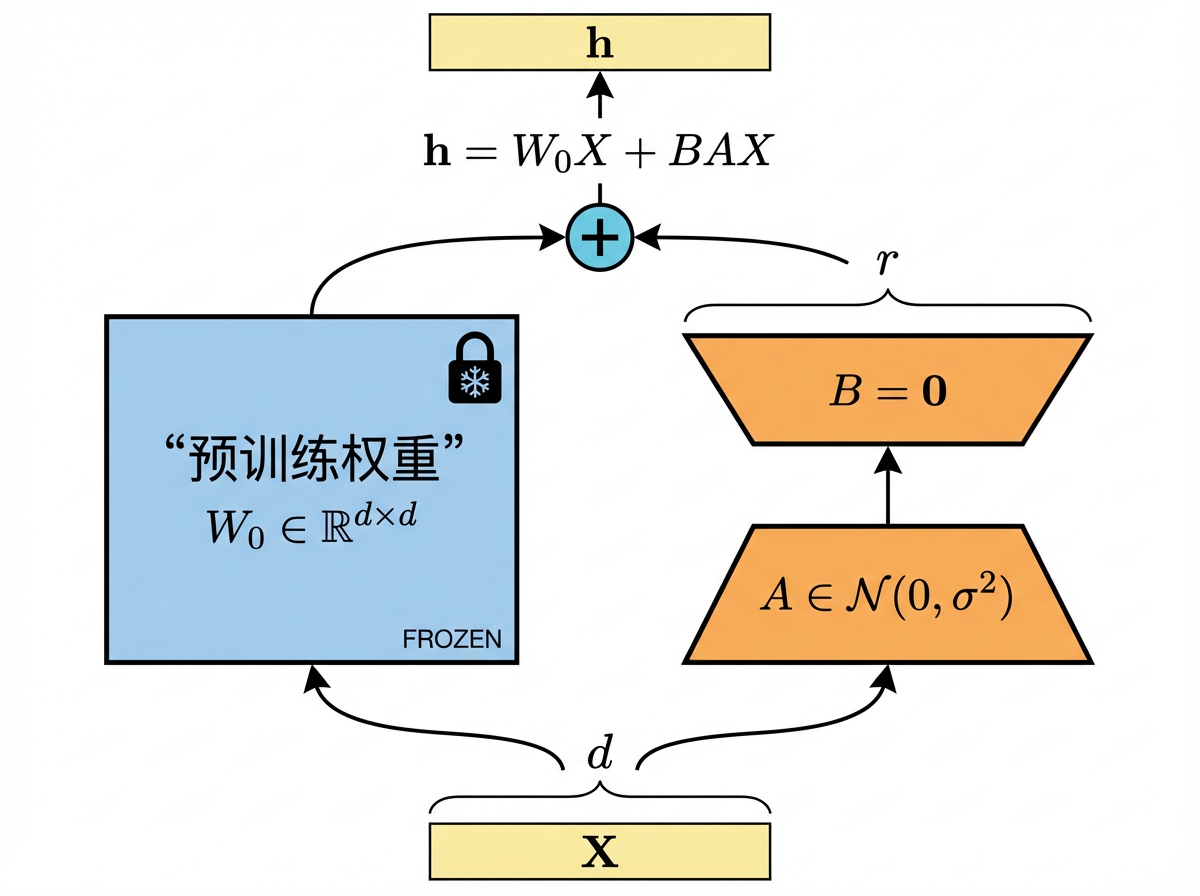
\includegraphics[width=0.75\textwidth]{figures/LoRA方法结构图.png}
    \caption{LoRA 方法结构示意图}
    \label{fig:lora-structure}
\end{figure}

在 LoRA 框架下，原始预训练权重矩阵可记为 $W^{(0)}$，模型在适配下游任务时所需的权重变化记为 $\Delta W$。与全量微调直接优化完整权重增量不同，LoRA 将该增量分解为两个可训练低秩矩阵的乘积，以低秩形式近似表示任务相关参数更新，即
\begin{equation}
W_{\text{new}} = W^{(0)} + \Delta W = W^{(0)} + BA ,
\label{eq:lora_weight_update}
\end{equation}
式中，$A$ 与 $B$ 表示在微调阶段参与训练的低秩矩阵，其秩 $r$ 通常远低于原始权重矩阵的维度。模型训练时只更新这两个新增矩阵，用它们刻画下游任务所需的参数增量，而预训练模型中的原始权重仍保持冻结状态。

在前向计算阶段，LoRA 会在原始线性映射结果的基础上加入低秩适配分支，使模型输出同时包含预训练权重贡献和任务增量贡献，其形式可写为
\begin{equation}
y = W^{(0)}x + \Delta Wx = W^{(0)}x + \frac{\alpha}{r}BAx ,
\label{eq:lora_forward}
\end{equation}
其中，$\alpha$ 用于控制低秩增量项在最终输出中的作用强度，$r$ 表示低秩矩阵的秩，用于对增量分支进行尺度归一化。这种设计使模型无需改变原始预训练参数，也能够通过低秩增量学习获得面向下游任务的适配能力。

因此，LoRA 的关键优势在于将微调目标从“大规模权重整体更新”转化为“少量新增低秩参数优化”，从而降低参数更新规模。从训练成本角度看，LoRA 只需优化附加的低秩矩阵，因此可训练参数规模和微调阶段的显存需求均明显低于全量微调。与此同时，原始预训练权重在训练过程中不被直接更新，有助于保留基座模型已有的通用语言能力，并在一定程度上减轻灾难性遗忘风险。已有研究表明，相比传统全量微调，LoRA 通过更新较少比例的参数，也能够在多个自然语言处理任务中达到接近全量微调的效果\cite{Hu2022LoRA}。因此，它为大语言模型在资源受限环境中的适配提供了一个轻量且实用的解决方案。

在 LoRA 方法之后，QLoRA（Quantized LoRA）进一步将量化技术引入参数高效微调过程。该方法在保留 LoRA 低秩适配思想的基础上，对预训练模型权重采用低比特表示，从而在尽可能维持模型任务性能的同时，进一步降低微调过程中的显存需求\cite{Dettmers2023QLoRA}。具体来看，QLoRA 采用 4-bit NormalFloat（NF4）作为权重量化表示形式，并利用双重量化（double quantization）进一步压缩量化过程中产生的常量信息。经过量化处理后，基座模型的预训练权重以较低精度形式保存且保持冻结，任务相关参数更新则主要由 LoRA 适配器承担。

在前向传播阶段，QLoRA 的输出可以理解为两部分的叠加：一部分来自经过双重量化恢复后的量化基座模型权重，另一部分来自 LoRA 适配器所学习的低秩增量。其计算形式可写为
\begin{equation}
Y^{\mathrm{BF16}}
=
X^{\mathrm{BF16}}
\operatorname{doubleDequant}
\left(
c_1^{\mathrm{FP32}},
c_2^{\mathrm{NF4}},
W^{\mathrm{NF4}}
\right)
+
X^{\mathrm{BF16}}A^{\mathrm{BF16}}B^{\mathrm{BF16}},
\label{eq:qlora_forward}
\end{equation}
式中，$W^{\mathrm{NF4}}$ 表示以 NF4 形式保存的预训练权重，$c_1$ 和 $c_2$ 分别对应量化过程中使用的常数项，$\operatorname{doubleDequant}(\cdot)$ 用于表示由双重量化到可计算权重形式的恢复过程。

双重量化的作用在于对量化常数本身再次进行压缩表示，并在计算时逐级恢复相应权重。该过程可进一步表示为
\begin{equation}
W^{\mathrm{BF16}}
=
\operatorname{doubleDequant}
\left(
c_1^{\mathrm{FP32}},
c_2^{\mathrm{NF4}},
W^{\mathrm{NF4}}
\right)
=
\operatorname{dequant}
\left(
\operatorname{dequant}
\left(
c_1^{\mathrm{FP32}},
c_2^{\mathrm{NF4}}
\right),
W^{\mathrm{NF4}}
\right),
\label{eq:double_dequant}
\end{equation}
其中，单次反量化可以写为
\begin{equation}
W^{\mathrm{FP32}}
=
\operatorname{dequant}(c^{\mathrm{FP32}}, W^{\mathrm{Int4}})
=
c^{\mathrm{FP32}} W^{\mathrm{Int4}} .
\label{eq:dequant}
\end{equation}

与原始 LoRA 相比，QLoRA 在参数更新规模较小的基础上进一步压缩了模型权重存储和训练显存需求，因此更适合在消费级显卡或资源受限计算环境中进行模型适配。由 LoRA 到 QLoRA 的发展表明，参数高效微调技术已从减少可训练参数，进一步延伸到降低显存占用和部署成本。对于本文研究的领域知识抽取任务而言，该类方法能够缓解大语言模型训练和本地部署中的资源压力，并为后续构建面向轻量化场景的可控知识抽取模型提供方法基础。

\section{本章小结}

本章从知识图谱相关理论、知识抽取相关技术以及大语言模型相关技术三个方面梳理了本文研究所需的理论基础与关键方法，为后续章节展开具体方法设计、实验验证与系统实现提供支撑。
